\documentclass[letter,11pt]{article}
\usepackage[margin=1.5cm]{geometry}
\usepackage{latexsym}
\usepackage{amsmath}
\usepackage{color}
\usepackage{graphicx}
\usepackage{amssymb}
\usepackage{alltt}
\usepackage{enumitem}
\usepackage{siunitx}
\usepackage{physics}
\usepackage{bm}
\usepackage{upgreek}
\usepackage{float}

\newenvironment{solution}{
    \vspace{0.16in} {\bf Solution:}
    
}{
	\vspace{0.16in}
}
\newcommand{\inti}[4]{
	\int_{#1}^{#2} #3 \, \mathrm{d} #4
}
\newcommand{\intii}[7]{
	\int_{#1}^{#2} \int_{#3}^{#4} #5 \, \mathrm{d} #6 \, \mathrm{d} #7
}
\newcommand{\expected}[1]{
    \mathbb{E}[#1]
}
\DeclareMathOperator*{\argmax}{arg\,max}
\DeclareMathOperator*{\argmin}{arg\,min}

%------------------------------------------------------

\begin{document}

\begin{center}
    {\bf \Large Math 189R problem set 2} \\
    \vspace{0.1in}
    Adam Guo \quad 2020-02-10
\end{center}

\begin{enumerate}
    \item \textbf{(Murphy 8.3)} Gradient and Hessian of the log-likelihood for logistic regression.

    \textit{Hint:} Use the \textbf{negative} log-likelihood of logistic regression for this problem.

    \begin{enumerate}
        \item Let $\sigma(x) = \frac{1}{1 + e^{-x}}$ be the sigmoid function. Show that \[\sigma'(x) = \sigma(x) [1 - \sigma(x)]\]

        \begin{solution}
            $\begin{aligned}
                \sigma'(x) &= \dv{x} \left[ \frac{1}{1 + e^{-x}} \right] \\
                    &= -\frac{-e^{-x}}{(1 + e^{-x})^2} \\
                    &= \frac{e^{-x}}{(1 + e^{-x})^2} \\
                \sigma(x) [1 - \sigma(x)] &= \frac{1}{1 + e^{-x}} \left( 1 - \frac{1}{1 + e^{-x}} \right) \\
                    &= \frac{1}{1 + e^{-x}} - \left( \frac{1}{1 + e^{-x}} \right)^2 \\
                    &= \frac{e^{-x}}{(1 + e^{-x})^2}
            \end{aligned}$

            Thus $\sigma'(x) = \sigma(x) [1 - \sigma(x)]$.
        \end{solution}

        \item Using the previous result and the chain rule of calculus, derive an expression for the gradient of the log likelihood for logistic regression.

        \begin{solution}
            By Murphy, \[\text{NLL}(\textbf{w}) = -\sum_{i=1}^N [y_i \log \mu_i + (1 - y_i) \log (1 - \mu_i)]\] where $\mu_i = \sigma(\textbf{w}^T \textbf{x}_i)$.

            \begin{align*}
                \text{NLL}({\textbf{w}}) &= -\sum_{i=1}^N [y_i \log \sigma(\textbf{w}^T \textbf{x}_i) + (1 - y_i) \log (1 - \sigma(\textbf{w}^T \textbf{x}_i))] \\
                \nabla \text{NLL}(\textbf{w}) &= -\sum_{i=1}^N \left[y_i \frac{\sigma'(\textbf{w}^T \textbf{x}_i) \textbf{x}_i}{\sigma(\textbf{w}^T \textbf{x}_i)} + (1 - y_i) \left( \frac{-\sigma'(\textbf{w}^T \textbf{x}_i) \textbf{x}_i}{1 - \sigma(\textbf{w}^T \textbf{x}_i)} \right) \right] \\
                    &= -\sum_{i=1}^N \left[ y_i \frac{\sigma(\textbf{w}^T \textbf{x}_i)[1 - \sigma(\textbf{w}^T \textbf{x}_i)]}{\sigma(\textbf{w}^T \textbf{x}_i)} \textbf{x}_i + (1 - y_i) \left( \frac{-\sigma(\textbf{w}^T \textbf{x}_i) [1 - \sigma(\textbf{w}^T \textbf{x}_i)]}{1 - \sigma(\textbf{w}^T \textbf{x}_i)} \right) \textbf{x}_i \right] \\
                    &= -\sum_{i=1}^N \left[ y_i (1 - \sigma(\textbf{w}^T \textbf{x}_i)) \textbf{x}_i + (1 - y_i) (-\sigma(\textbf{w}^T \textbf{x}_i)) \textbf{x}_i \right] \\
                    &= -\sum_{i=1}^N y_i \textbf{x}_i - \sigma(\textbf{w}^T \textbf{x}_i) \textbf{x}_i \\
                    &= \sum_{i=1}^N (\mu_i - y_i) \textbf{x}_i \\
                    &= \textbf{X}^T (\bm{\mu} - \textbf{y})
            \end{align*}
        \end{solution}

        \item The Hessian can be written as $\textbf{H} = \textbf{X}^T \textbf{SX}$ where $\textbf{S} = \text{diag}(\mu_1 (1 - \mu_1), \dots, \mu_n (1 - \mu_n))$. Derive this and show that $\textbf{H} \succeq 0$ ($A \succeq 0$ means that $A$ is positive semidefinite).

        \begin{solution}
            \begin{align*}
                \mathbf{H} = \nabla (\nabla \text{NLL}(\mathbf{w}))^T &= \nabla (\mathbf{X}^T (\bm{\mu} - \mathbf{y}))^T \\
                    &= \nabla (\mathbf{X}^T \bm{\mu} - \mathbf{X}^T \mathbf{y})^T \\
                    &= \nabla (\bm{\mu}^T \mathbf{X}) \\
                    &= \nabla \left(\sum_{i} \mu_i\right) \mathbf{x}_i \quad \text{where } \mathbf{x}_i \text{ denotes the columns of } \mathbf{X} \\
                    &= \left(\sum_i \nabla \mu_i\right) \mathbf{x}_i \\
                    &= \left(\sum_i \nabla \sigma(\mathbf{x}_i^T \mathbf{w})\right) \mathbf{x}_i \\
                    &= \left(\sum_i \mu_i (1 - \mu_i) \right) \mathbf{x}_i \mathbf{x}_i^T \\
                    &= \mathbf{X}^T \mathbf{S} \mathbf{X}
            \end{align*}

            The eigenvalues of $\mathbf{H}$ are given by $\mathbf{S}$. Since $\mathbf{H}$ is positive semidefinite iff its eigenvalues are non-negative, $\mathbf{H}$ is positive semidefinite iff $\mathbf{S}$ is positive semidefinite.

            $\mu_i = \sigma(\mathbf{w}^T \mathbf{x}_i)$. By definition, $\sigma \in (0, 1)$. Hence, $\mu_i \in (0, 1)$ and $(1 - \mu_i) \in (0, 1)$. Hence, $\mu_i (1 - \mu_i) \geq 0$. Thus, $\mathbf{S}$ and hence $\mathbf{H}$ are positive semidefinite.


        \end{solution}
    \end{enumerate}

    \newpage

    %----------------------------------

    \item \textbf{(Murphy 2.11)} Derive the normalisation constant ($Z$) for a one dimensional zero-mean Gaussian \[\mathbb{P}(x; \sigma^2) = \frac{1}{Z} \exp(-\frac{x^2}{2\sigma^2})\] such that $\mathbb{P}(x; \sigma^2)$ becomes a valid density.

    \begin{solution}
        \begin{align*}
            \inti{-\infty}{\infty}{\frac{1}{Z} \exp(\frac{-x^2}{2\sigma^2})}{x} &= 1 \\
            \left(\inti{-\infty}{\infty}{\exp(\frac{-x^2}{2\sigma^2})}{x}\right)^2 &= Z^2
        \end{align*}
        
        We use this expression for $Z^2$ to integrate in polar coordinates.

        \begin{align*}
            Z^2 &= \inti{-\infty}{\infty}{\left(\inti{-\infty}{\infty}{\exp(\frac{-x^2}{2\sigma^2})}{x}\right) \exp(\frac{-y^2}{2\sigma^2})}{y} \\
                &= \inti{-\infty}{\infty}{\inti{-\infty}{\infty}{\exp(\frac{-x^2 - y^2}{2\sigma^2})}{x}}{y} \\
                &= \inti{0}{2\pi}{\inti{0}{\infty}{\exp(\frac{-r^2}{2\sigma^2}) r}{r}}{\theta}
            \intertext{Let $u = r^2$. $\dd{u} = 2r \dd{r}$.}
            Z^2 &= \frac{1}{2} \inti{0}{2\pi}{\inti{0}{\infty}{\exp(\frac{-u}{2\sigma^2})}{u}}{\theta} \\
                &= \frac{1}{2} \inti{0}{2\pi}{-2 \sigma^2}{\theta} \\
                &= 2\pi\sigma^2 \\
            Z   &= \sqrt{2\pi} \sigma
        \end{align*}
    \end{solution}

    \newpage

    %----------------------------------

    \item \textbf{(regression)} In this problem, we will use the online news popularity dataset to set up a model for linear regression. In the starter code, we have already parsed the data for you. However, you might need internet connection to access the data and therefore successfully run the starter code.

    We split the csv file into a training and test set with the first two thirds of the data in the training set and the rest for testing. Of the testing data, we split the first half into a "validation set" (used to optimise hyperparameters while leaving your testing data pristine) and the remaining half as your test set. We will use this data for the remainder of the problem. The goal of this data is to predict the \textbf{log} number of shares a news article will have given the other features.

    \begin{enumerate}
        \item \textbf{(math)} Show that the maximum a posteriori problem for linear regression with a zero-mean Gaussian prior $\mathbb{P}(\textbf{w}) = \prod_j \mathcal{N}(w_j \mid 0, \tau^2)$ on the weights, \[\argmax_{\textbf{w}} \sum_{i=1}^N \log \mathcal{N}(y_i \mid w_0 + \textbf{w}^T \textbf{x}_i, \sigma^2) + \sum_{j=1}^D \log \mathcal{N}(w_j \mid 0, \tau^2)\] is equivalent to the ridge regression problem \[\argmin \frac{1}{N} \sum_{i=1}^N (y_i - (w_0 + \textbf{w}^T \textbf{x}_i))^2 + \lambda ||w||_2^2\] with $\lambda = \sigma^2/\tau^2$.

        \begin{solution}
            \begin{align*}
                &\quad\: \argmax_{\textbf{w}} \sum_{i=1}^N \log \mathcal{N}(y_i \mid w_0 + \textbf{w}^T \textbf{x}_i, \sigma^2) + \sum_{j=1}^D \log \mathcal{N}(w_j \mid 0, \tau^2) \\
                &= \argmax_{\textbf{w}} \sum_{i=1}^N \log \left( \frac{1}{\sqrt{2\pi}\sigma} e^{-\frac{(y_i - (w_0 + \mathbf{w}^T \mathbf{x}_i))^2}{2\sigma^2}} \right) + \sum_{j=1}^D \log \left( \frac{1}{\sqrt{2\pi}\tau} e^{-\frac{w_j^2}{2\tau^2}} \right) \\
                &= \argmax_{\textbf{w}} \sum_{i=1}^N \left(\log \frac{1}{\sqrt{2\pi}\sigma} - \frac{(y_i - (w_0 + \mathbf{w}^T \mathbf{x}_i))^2}{2\sigma^2}\right) + \sum_{j=1}^D \left( \log\frac{1}{\sqrt{2\pi}\tau} - \frac{w_j^2}{2\tau^2} \right) \\
                &= \argmax_{\textbf{w}} \log \frac{1}{(\sqrt{2\pi}\sigma)^N} + \log \frac{1}{(\sqrt{2\pi}\tau)^D} - \left(\sum_{i=1}^N \frac{(y_i - (w_0 + \mathbf{w}^T \mathbf{x}_i))^2}{2\sigma^2} + \frac{||w||_2^2}{2\tau^2} \right)
            \end{align*}

            Since the first two constant log terms do not affect the optimisation problem, this is equivalent to minimising the summation term that is being subtracted. Hence, this is equivalent to

            \begin{align*}
                &\quad\: \argmin_{\mathbf{w}} \sum_{i=1}^N \frac{(y_i - (w_0 + \mathbf{w}^T \mathbf{x}_i))^2}{2\sigma^2} + \frac{||w||_2^2}{2\tau^2} \\
                &= \argmin_{\mathbf{w}} \frac{1}{2\sigma^2} \left( \sum_{i=1}^N (y_i - (w_0 + \mathbf{w}^T \mathbf{x}_i))^2 + \frac{\sigma^2||w||_w^2}{\tau^2} \right)
            \end{align*}

            Multiplying by a constant term $2\sigma^2$ and letting $\lambda = \frac{\sigma^2}{\tau^2}$, this is thus equivalent to the ridge regression problem

            \begin{align*}
                &\quad\: \argmin_{\mathbf{w}} \sum_{i=1}^N (y_i - (w_o + \mathbf{w}^T \mathbf{x}_i))^2 + \lambda ||w||_2^2
            \end{align*}
        \end{solution}

        \item \textbf{(math)} Find a closed form solution $\textbf{x}^*$ to the ridge regression problem: \[\text{minimise: } ||A\textbf{x} - \textbf{b}||_2^2 + ||\Gamma \textbf{x}||_2^2\]

        \begin{solution}
            \begin{align*}
                \nabla (||A\mathbf{x} - \mathbf{b}||_2^2 + ||\Gamma\mathbf{x}||_2^2) &= \nabla((A\mathbf{x} - \mathbf{b})^T (A\mathbf{x} - \mathbf{b}) + (\Gamma\mathbf{x})^T (\Gamma\mathbf{x})) \\
                    &= \nabla ((\mathbf{x}^T A^T - \mathbf{b}^T)(A\mathbf{x} - \mathbf{b}) + (\mathbf{x}^T\Gamma^T)(\Gamma\mathbf{x})) \\
                    &= \nabla(\mathbf{x}^TA^TA\mathbf{x} - \mathbf{x}^TA^T\mathbf{b} - \mathbf{b}^TA\mathbf{x} + \mathbf{b}^T\mathbf{b} + \mathbf{x}^T\Gamma^T\Gamma\mathbf{x}) \\
                    &= 2A^TA\mathbf{x} - 2A^T\mathbf{b} + 2\Gamma^T\Gamma\mathbf{x}
                \intertext{To optimise, let the gradient equal 0.}
                2A^T\mathbf{b} &= 2A^TA\mathbf{x}^* + 2\Gamma^T\Gamma\mathbf{x}^* \\
                A^T\mathbf{b} &= (A^TA + \Gamma^T\Gamma)\mathbf{x}^* \\
                \mathbf{x}^* &= (A^TA + \Gamma^T\Gamma)^{-1}A^T\mathbf{b}
                \intertext{yielding the solution for $\mathbf{x}^*$.}
            \end{align*}
        \end{solution}

        \item \textbf{(implementation)} Attempt to predict the log shares using ridge regression from the previous problem solution. Make sure you include a bias term and \textit{don't regularise the bias term}. Find the optimal regularisation parameter $\lambda$ from the validation set. Plot both $\lambda$ versus the validation RMSE (you should have tried at least 150 parameter settings randomly chosen between 0.0 and 150.0 because the dataset is small) and $\lambda$ versus $||\theta^*||_2$ where $\theta$ is your weight vector. What is the final RMSE on the test set with the optimal $\lambda^*$?

        \begin{solution}
            \begin{figure}[h]
                \centering
                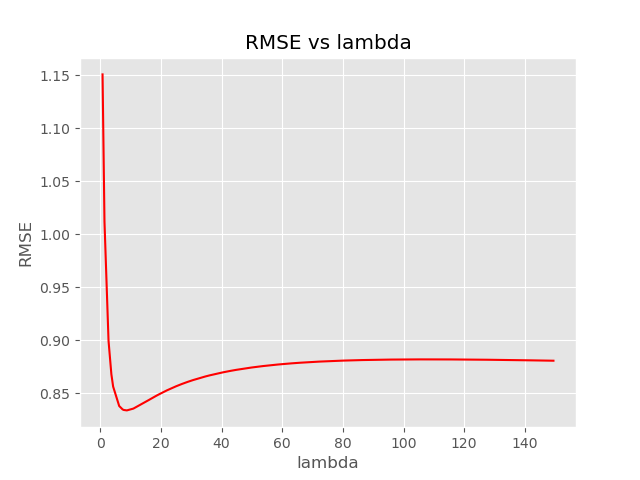
\includegraphics[width=10cm]{RMSE_vs_lambda.png}
            \end{figure}

            \begin{figure}[H]
                \centering
                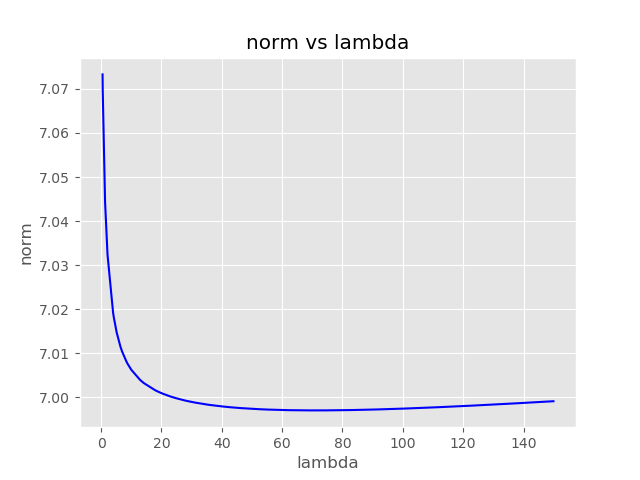
\includegraphics[width=10cm]{norm_vs_lambda.png}
            \end{figure}

            The optimal regularisation parameter is $\lambda = 9.1326$, with RMSE of 0.8341 on the validation set and 0.8628 on the test set.
        \end{solution}

        \item \textbf{(math)} Consider regularised linear regression where we pull the basis term out of the feature vectors. That is, instead of computing $\hat{\textbf{y}} = \theta^T \textbf{x}$ with $\textbf{x}_0 = 1$, we compute $\hat{\textbf{y}} = \theta^T \textbf{x} + b$. This corresponds to solving the optimisation problem \[\text{minimise: } ||A\textbf{x} + b\textbf{1} - \textbf{y}||^2_2 + ||\Gamma \textbf{x}||_2^2\] Solve for the optimal $\textbf{x}^*$ explicitly. Use this closed form to compute the bias term for the previous problem (with the same regularisation strategy). Make sure it is the same.

        \begin{solution}
            Suppose $\mathbf{1}$ has length $n$.

            \begin{align*}
                &\quad\: ||A\mathbf{x} + b\mathbf{1} - \mathbf{y}||_2^2 + ||\Gamma\mathbf{x}||_2^2 \\
                &= (A\mathbf{x} + b\mathbf{1} - \mathbf{y})^T(A\mathbf{x} + b\mathbf{1} - \mathbf{y}) + (\Gamma\mathbf{x})^T(\Gamma\mathbf{x}) \\
                &= (\mathbf{x}^TA^T + b\mathbf{1}^T - \mathbf{y}^T)(A\mathbf{x} + b\mathbf{1} - \mathbf{y}) + \mathbf{x}^T\Gamma^T\Gamma\mathbf{x} \\
                &= \mathbf{x}^TA^TA\mathbf{x} + \mathbf{x}^TA^Tb\mathbf{1} - \mathbf{x}^TA^T\mathbf{y} + b\mathbf{1}^TA\mathbf{x} + b^2\mathbf{1}^T\mathbf{1} - b\mathbf{1}^T\mathbf{y} - \mathbf{y}^TA\mathbf{x} - b\mathbf{y}^T\mathbf{1} + \mathbf{y}^T\mathbf{y} + \mathbf{x}^T\Gamma^T\Gamma\mathbf{x} \\
                &= \mathbf{x}^TA^TA\mathbf{x} + 2b\mathbf{1}^TA\mathbf{x} - 2\mathbf{y}^TA\mathbf{x} - 2b\mathbf{1}^T\mathbf{y} + nb^2 + \mathbf{y}^T\mathbf{y} + \mathbf{x^T}\Gamma^T\Gamma\mathbf{x}
            \end{align*}

            Need to optimise both $\mathbf{x}$ and $b$.

            \begin{align*}
                \nabla_b (||A\mathbf{x} + b\mathbf{1} - \mathbf{y}||_2^2 + ||\Gamma\mathbf{x}||_2^2) &= 2\mathbf{1}^TA\mathbf{x} - 2\mathbf{1}^T\mathbf{y} + 2bn
                \intertext{Setting $\nabla_b = 0$,}
                b^* &= \frac{1}{n}\mathbf{1}^T(\mathbf{y} - A\mathbf{x})
            \end{align*}

            Using $b^*$ to optimise $x$,

            \begin{align*}
                \nabla_x (||A\mathbf{x} + b\mathbf{1} - \mathbf{y}||_2^2 + ||\Gamma\mathbf{x}||_2^2) &= 2A^TA\mathbf{x} + 2bA^T\mathbf{1} - 2A^T\mathbf{y} + 2\Gamma^T\Gamma\mathbf{x} \\
                    &= 2A^TA\mathbf{x} + 2\frac{\mathbf{1}^T(\mathbf{y} - A\mathbf{x})}{n}A^T\mathbf{1} - 2A^T\mathbf{y} + 2\Gamma^T\Gamma\mathbf{x}
            \end{align*}

            Setting $\nabla_x = 0$,

            \begin{align*}
                0 &= (A^TA + \Gamma^T\Gamma)\mathbf{x}^* + \frac{1}{n}\mathbf{1}^T(\mathbf{y} - A\mathbf{x}^*)A^T\mathbf{1} - A^T\mathbf{y} \\
                    &= (A^TA + \Gamma^T\Gamma)\mathbf{x}^* + \frac{1}{n}\mathbf{1}^T\mathbf{y}A^T\mathbf{1} - \frac{1}{n}\mathbf{1}^TA\mathbf{x}^*A^T\mathbf{1} -  A^T\mathbf{y} \\
                    &= (A^TA + \Gamma^T\Gamma)\mathbf{x}^* + \frac{1}{n}A^T\mathbf{1}\mathbf{1}^T\mathbf{y} - \frac{1}{n}A^T\mathbf{1}\mathbf{1}^TA\mathbf{x}^* - A^T\mathbf{y} \\
                    &= (A^TA + \Gamma^T\Gamma - \frac{1}{n}A^T\mathbf{1}\mathbf{1}^TA)\mathbf{x}^* + (\frac{1}{n}A^T\mathbf{1}\mathbf{1}^T - A^T)\mathbf{y} \\
            \end{align*}

            \begin{align*}
                (A^TA + \Gamma^T\Gamma - \frac{1}{n}A^T\mathbf{1}\mathbf{1}^TA)\mathbf{x}^* &= (-\frac{1}{n}A^T\mathbf{1}\mathbf{1}^T + A^T)\mathbf{y} \\
                    &= A^T(\mathbf{I} - \frac{1}{n}\mathbf{1}\mathbf{1}^T)\mathbf{y}
            \end{align*}

            Hence, \[\mathbf{x}^* = (A^TA + \Gamma^T\Gamma - \frac{1}{n}A^T\mathbf{1}\mathbf{1}^TA)^{-1} A^T(\mathbf{I} - \frac{1}{n}\mathbf{1}\mathbf{1}^T)\mathbf{y}\] is the optimal solution for $\mathbf{x}^*$.
        \end{solution}

        \item \textbf{(implementation)} We can also compute the solution to the least squares problem using gradient descent. Consider the same bias-relocated objective \[\text{minimise: } f = ||A\textbf{x} + b\textbf{1} - \textbf{y}||_2^2 + ||\Gamma \textbf{x}||_2^2\] Compute the gradients and run gradient descent. Plot the $l_2$ norm between the optimal $(\textbf{x}^*, b^*)$ vector you computed in closed form and the iterates generated by gradient descent. Hint: your plot should move down and to the left and approach zero as the number of iterations increases. If it doesn't, try decreasing the learning rate.

        \begin{solution}
            \begin{figure}[h]
                \centering
                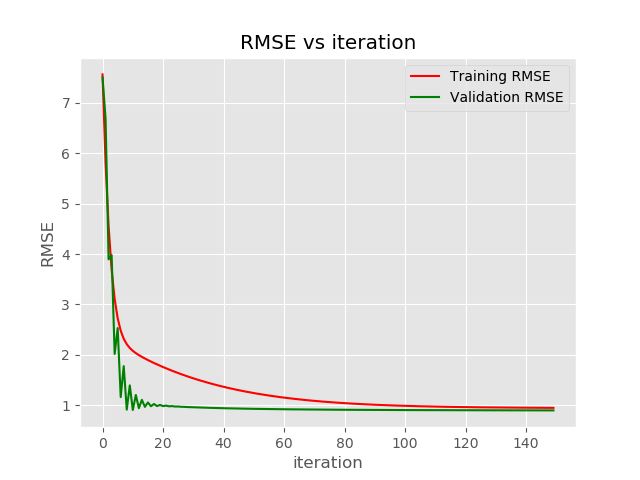
\includegraphics[width=10cm]{convergence.png}
            \end{figure}
        \end{solution}
    \end{enumerate}
\end{enumerate}

\end{document}